\documentclass[12pt]{article}
\usepackage{graphicx}
\usepackage{float}
\usepackage{amsmath}
\setlength{\parskip}{5mm}
\renewcommand{\baselinestretch}{1.0}

\title{Project Report 2 : 3D Shape Search Engine}
\author{Brian R. Cairl}
\begin{document}
\maketitle
\pagebreak

\newcommand{\ith}{i$^{th}$\hspace{0.5mm}}
\newcommand{\jth}{j$^{th}$\hspace{0.5mm}}
\newcommand{\st}{\hspace{0.5mm}:\hspace{0.5mm}}
\newcommand{\fa}{\hspace{0.5mm}\forall\hspace{0.5mm}}


\section*{Introduction}

	\noindent	
	This report details the design and testing of a 3D shape search engine which leverages several types of 3D shape descriptors. In particular, this search engine makes use of Geodesic distance (GD) and Euclidean distance (ED) shape descriptors (as well as a custom, curvature-base descriptor) to generate a pairwise similarity meaures (a \emph{distance}) between 3D meshes. The contents of this report will include a description of the code written to generate both GD and ED descriptors, given a 3D shape (mesh) input; a description of how noise and distortion were added to a set of 3D models (TOSCA data set); a description of how the search-engine was implimented, and a corresponding GUI front-end for 3D shape retrieval; and an experimental comparison between GD and ED based searches when clean, distorted and incomplete models are presented to the aforementioned search engine. Additionally, a tutorial will be provided as to how to run the search-engine GUI.

	\noindent	
	In addition to aforementioned project requirements, this report will also present the result of a custom feature descriptor when applied to 3D shape matching. This custom descriptor, dubbed the \emph{CD}, or curvature-dissimilarity descriptor, utilizes pair-wise dot products of unit normals which emenate from the triangular faces of each mesh. The formulation of this descriptor will be covered in detail at the end of this report, and will be compared to the performance of the GD and ED descriptors when applied to shape searching.


\section*{GD and ED Descriptors}
	
	\noindent
	Geodesic-distance (GD) and Euclidean Distance (ED) descriptors are histogram-based 3D descriptors used in the identification of 3D shapes. These descriptors are utilized to represent a 3D shape as high-dimensional feature vector. This section will describe the MATLAB implementation of a GD/ED descriptor generator used throughout this project.

	\noindent
	 GD and ED descriptors are generated using the MATLAB functions \emph{create\_GDdescriptor} and \emph{create\_EDdescriptor}, respectively. Each function takes a single mesh-structure argument, by default. The mesh structure contains two member variables which contain a list of vertices, $V$, and edge connections, $E$, respectively. Within each of these functions, correspnding GD and ED values are calculated between some percentage of the vertices (to all other vertices) within each mesh and binned using a function  \emph{bin\_values(d,dmin,dmax,dres)}, which creates a histogram (feature vector) from a vector of distances, $d$. Here we consider only a percentage of the mesh during feature-vector generation for the sake of saving computation time. The generated histogram has a minimum and maximum binning distance of $dmin$ and $dmax$; and a binning resolution of $dres$. Henceforth, distance values are counted into the \jth bin of each \ith histogram, $H_{j}^{i}$ as follows:
	\begin{equation}
    		H_{j}^{i} = 
		\sum_{d \in D \text{ and } d < \text{dmax}} u(d) : u(d) = 
		\begin{cases}
    		1,	& (\text{dmin} + \text{dres}*j) < d < (\text{dmin} + \text{dres}*(j+1))  \\
    		0,   & \text{otherwise}
		\end{cases}
	\end{equation}
	To clarify, each histogram,  $H_{j}^{i}$, is created using distances from the \ith vertex to \emph{all} other vertices in the provided mesh. Once histograms generated for each sample vertice, they are summed (in an element wise fashion) and then normalized by the number of sample vertexes considered in feature generation. We can, thus, wreite the final feature vector, $x\in\Re^{N}$, by:

	\begin{equation}
		x = \frac{1}{n_{\text{vectices}}}\sum_{i} H^{i}
	\end{equation}
	The dimensionality of $x$, $N$, is determined by :
	\begin{equation}
		N = \text{ceil}\left( \frac{\text{dmax} - \text{dmin} }{\text{dres}} \right)
	\end{equation}

	\noindent
	As for the distance calculations, seperate GD and ED functions have been written to handle the calculation of distance between a sample vertex and all other vertices in a mesh. To calculate the GD between points, a shortest path algorithm, $dijkstras(G,i)$ has been written which calculates theshortest  distance between a node, $i$, to all other nodes in a graph $G$, as well as the associated pathing information. The graph $G$ is represented as an adjacency matrix whose edge connections are computed as eucliden distances between connected nodes. The graph $G$ is generated from an input mesh $M$ by a seperate function \emph{mesh2graph(M,p)} which converts the mesh structure to the aforementioned adjaceny-matrix structure. The input parameter $p$ is used to set the order of the $L_{p}$-norm distance to be computed between each graph node. To compute the euclidean distance between points, $p$ is, obviously, set to $p=2$.
	
	\noindent
	To calculate the ED between points, an $L_{2}$ norm calculation performed on the vector difference between each \ith sample vertex and all other vertices of the mesh $M$. This calculation is performed from within the driver function, \emph{create\_EDdescriptor}, aa a helper subroutine, \emph{euclidean}.


	\subsection*{Distance measure for shape matching}

		\noindent
		During shape-matching process, the distance (scalar dissimilarity) between shapes is determined by the distance between associated feature vectors. For a pair of meshes $A$ and $B$ with associated feature vectors $x^{A}$ and $x^{B}$, shape dissimilarity, $d_{AB}$ is calculated by:

		\begin{equation}
			d_{AB} = \sqrt{ \sum_{i=0}^{N-1} \left( x^{A}_{i} - x^{B}_{i} \right)^{2} }
			\label{eq::shape_distance}
		\end{equation} 



\section*{Noise and Mesh Distortion simulation}
	
	\noindent
	For the purpose of testing the robustness of the ED and GD descriptors, and in-turn the 3D shape search-engine, the provided (reduced) TOSCA dataset is augmented with noisey and incomplete versions of the original clean models.

	\subsection*{Noisy Datasets}

		\noindent
		Noisy models are generated by adding Gaussian noise to each clean model in the original database. Each original mesh is modified using the provided function \emph{addGaussianNoise} for three levels of Gaussian noise. Therefore, three (low, med, high) noisy data models are generated for each clean model. Noise levels are chosen to be 0.001, 0.008 and 0.015 for the low, medium and high noise models respectively. Noisy mesh generation is automated with a script named \emph{noisy\_query\_set\_generation}, which generates new noisy models from each original, clean model for each level of noise. Figure \ref{fig::veryNoisyCat} shows a comparison between a clean and noisy model.

	\begin{figure}[!h]
		\centering
		\fbox{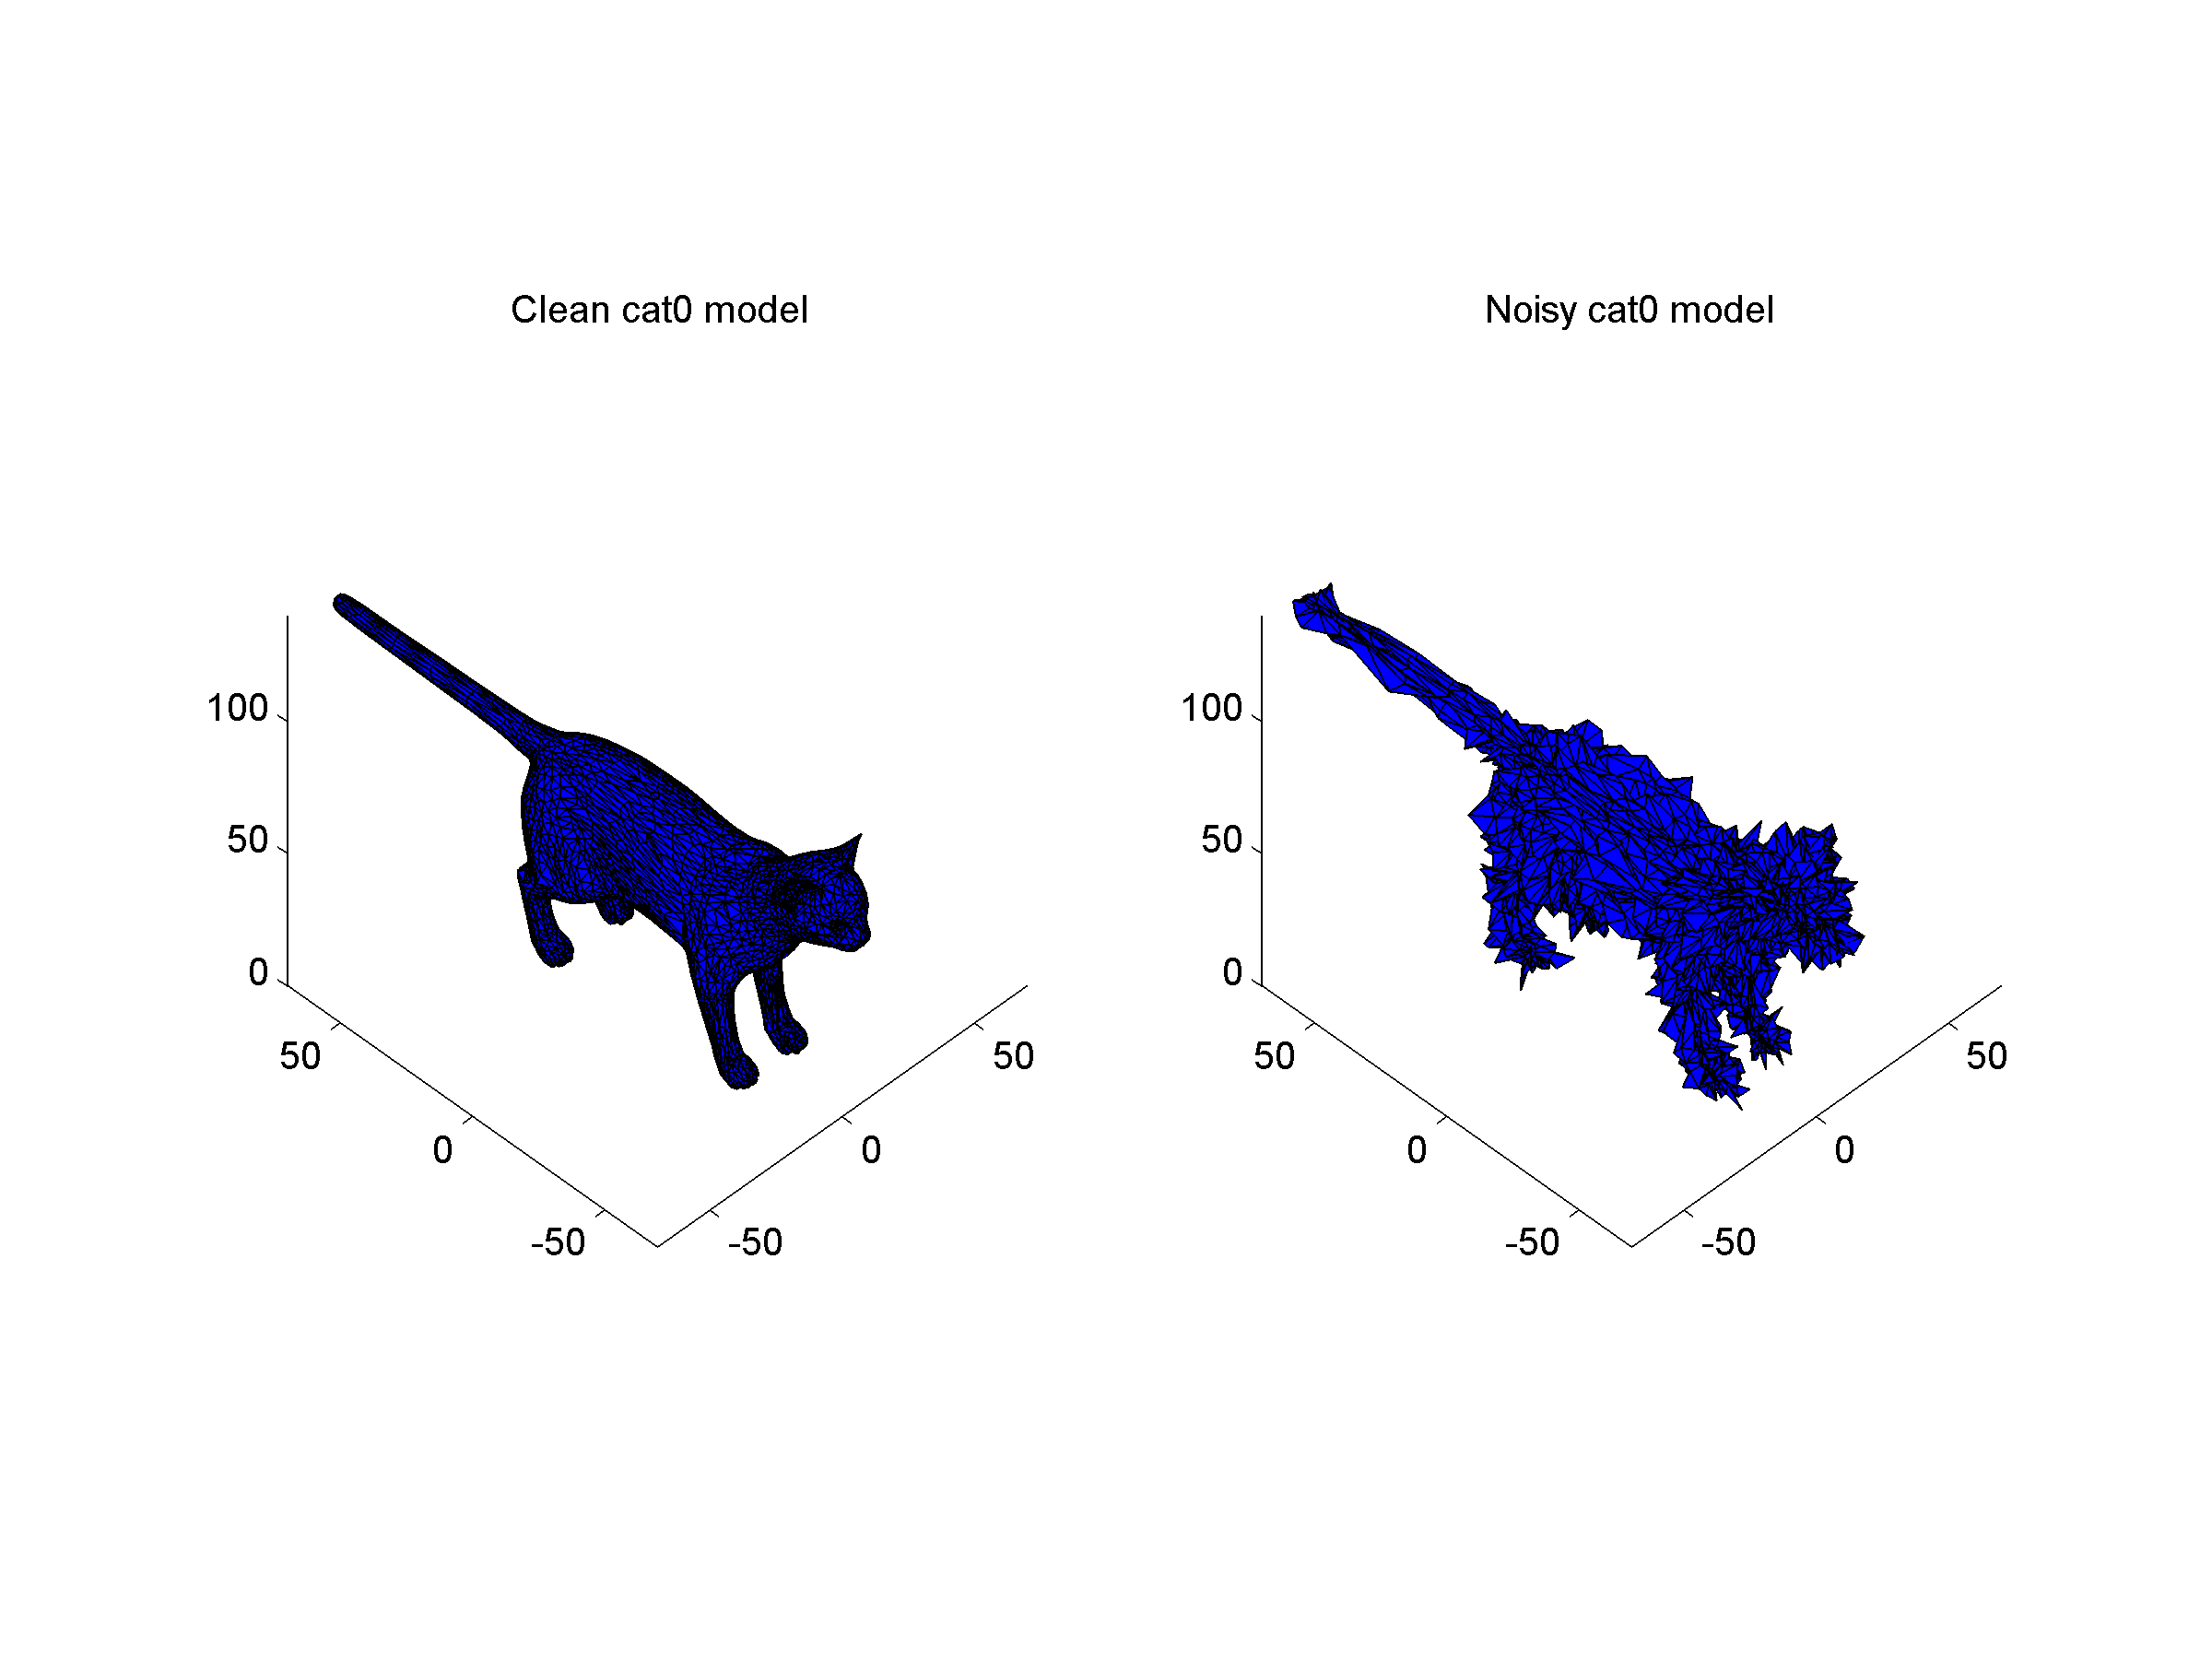
\includegraphics[width=\textwidth]{plots/noisy_clean.png}}
		\caption{Comparison of a clean and noisy model}
		\label{fig::veryNoisyCat}
	\end{figure}


	\subsection*{Incomplete Datasets}

		\noindent
		Three incomplete models are generated for each clean model by removing incrementally larger portions of each original mesh using the program MeshLab. Namely, low, medium, and highly effected models are generated by the aforementioned process. Any resulting holes in the effect mesh are filled using an hole-filling algorithm built into the MeshLab software. Figure \ref{fig::veryDeadCat} shows a comparison between a clean and incomplete model.
 
	\begin{figure}[!h]
		\centering
		\fbox{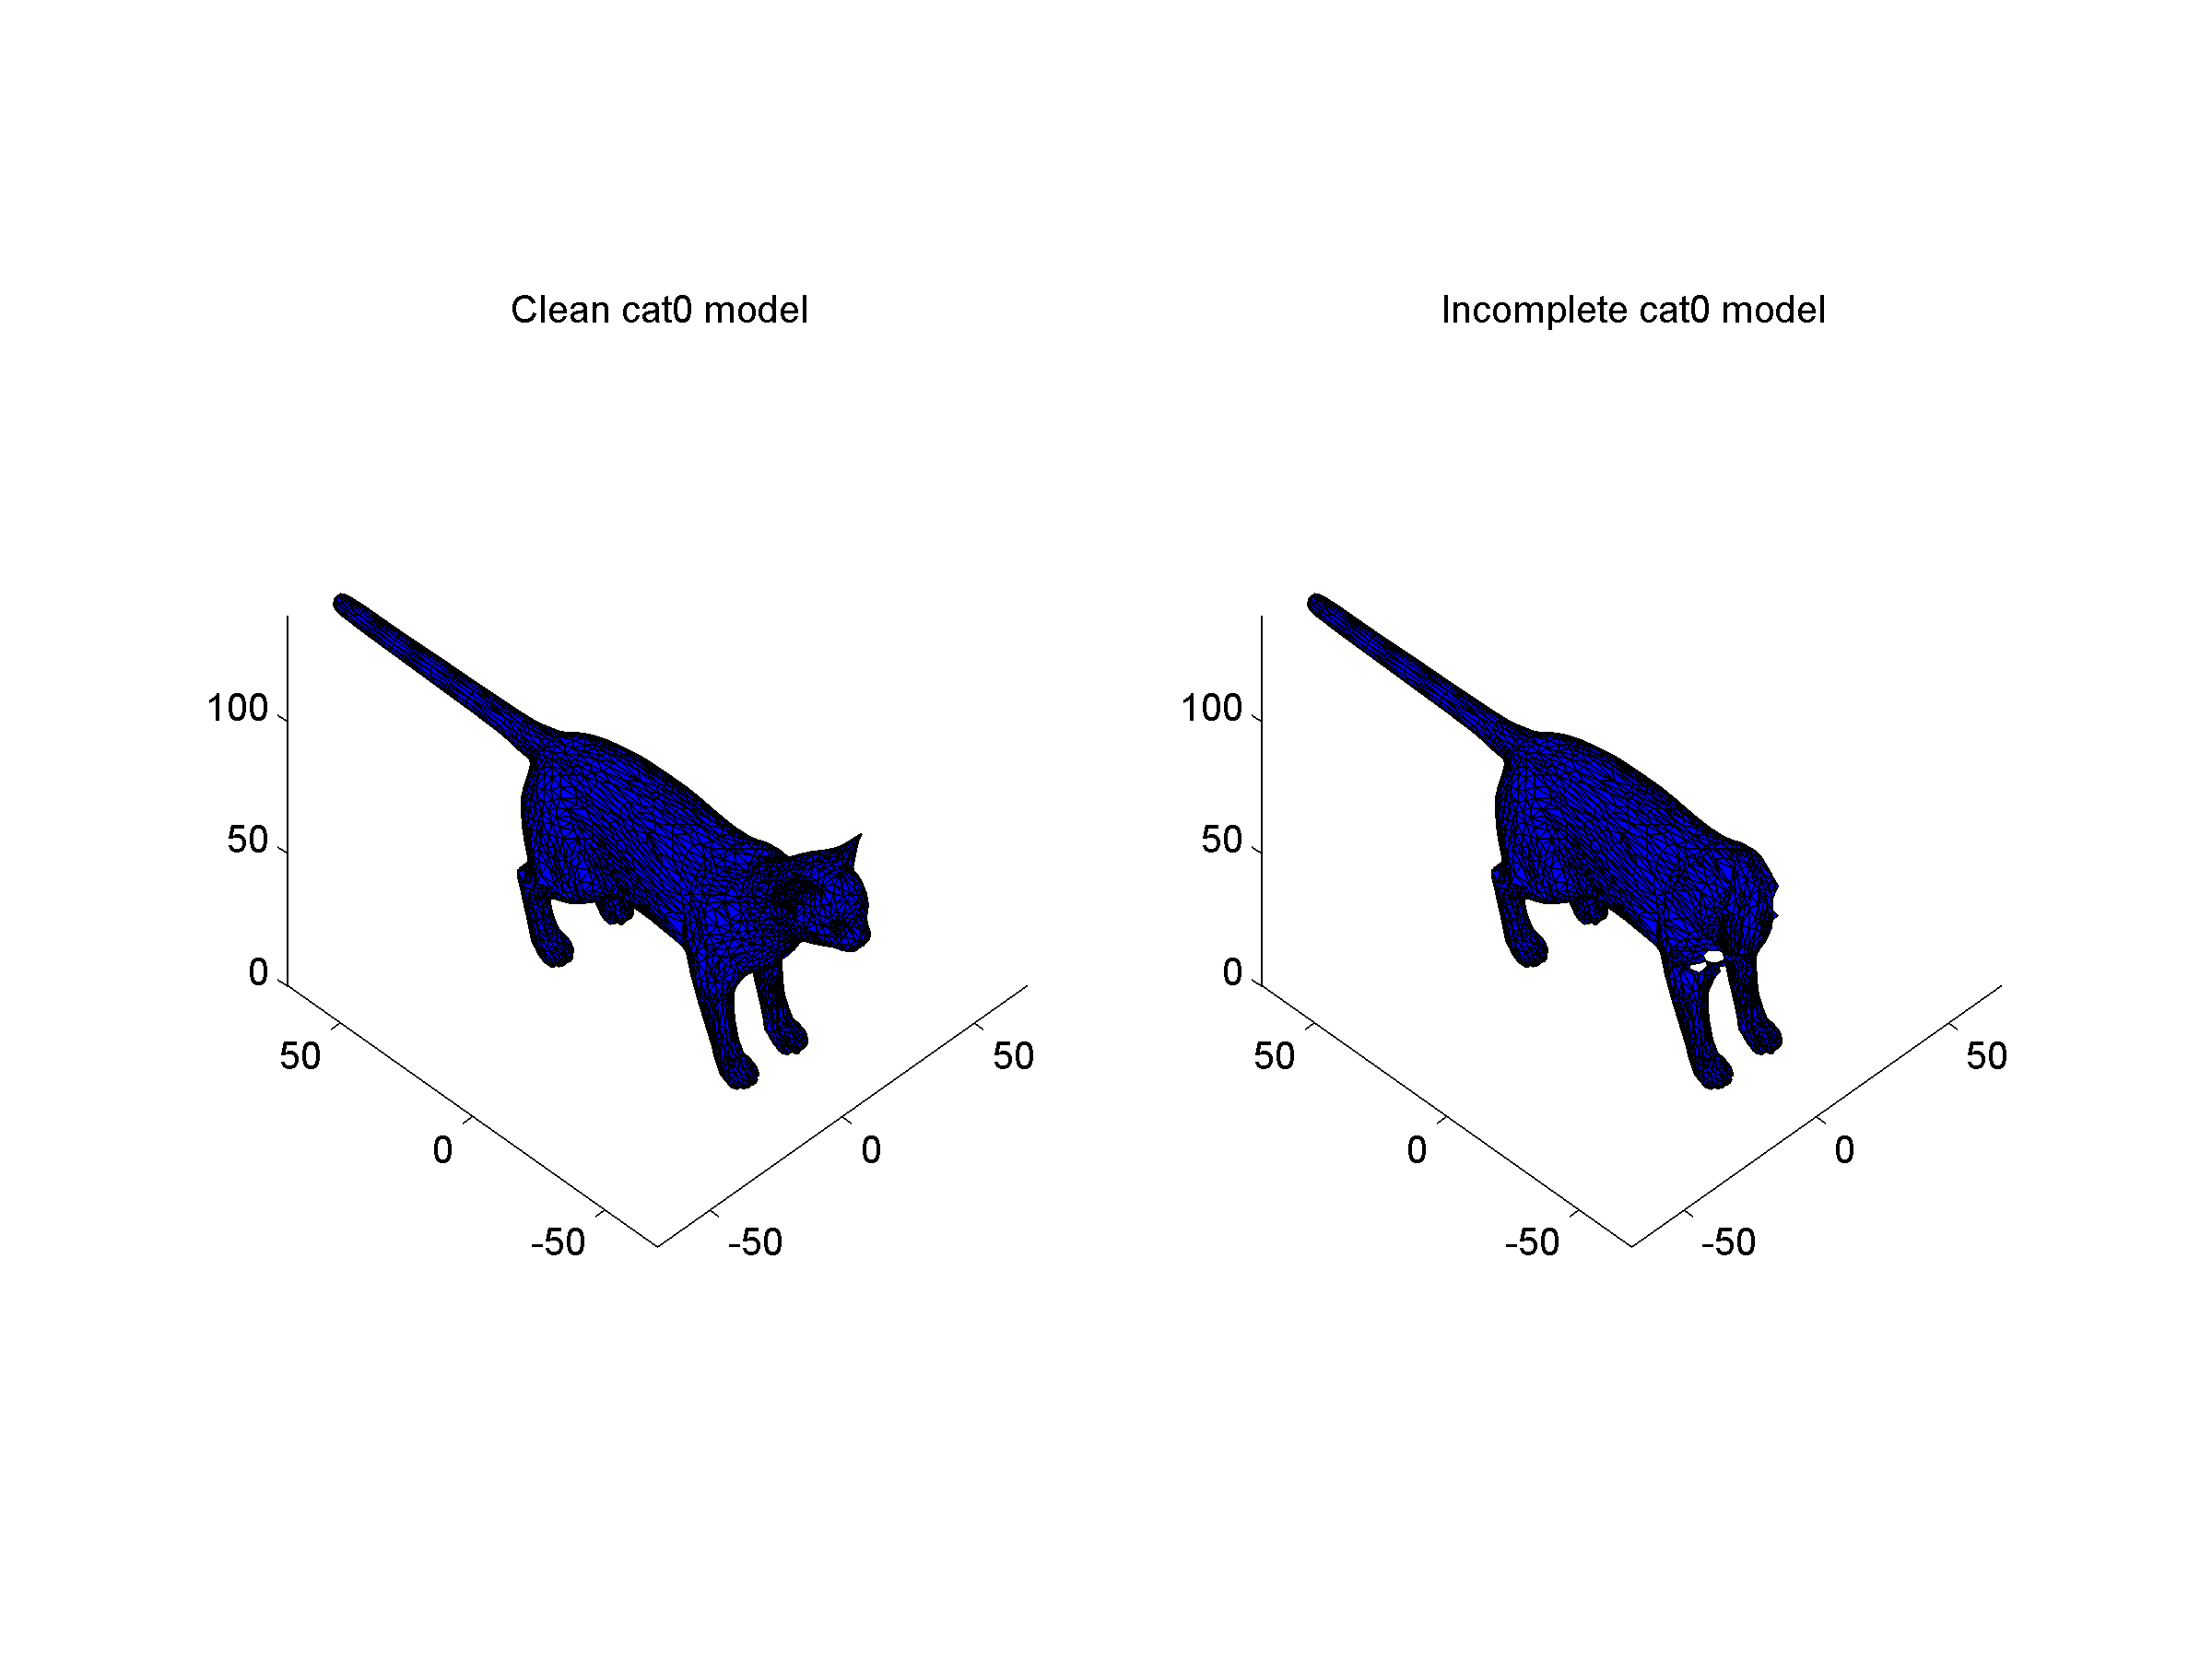
\includegraphics[width=\textwidth]{plots/incomp_clean.png}}
		\caption{Comparison of a clean and noisy model}
		\label{fig::veryDeadCat}
	\end{figure}


\section*{The 3D Shape Search Engine (and GUI)}

	\noindent


	\subsection*{How to run the Search Enginer GUI}



\section*{Search Engine Results}

	\noindent
	A script, \emph{search\_engine\_tester}, has been generated to automate perfomance tests for the generated search engine code. 




\section*{Concluding Remarks}



	\bibliography{refs}{}
	\bibliographystyle{plain}

\end{document}